
Create a \emph{transparent} benchmark for methods of Reinforcement Learning in Healthcare

\section{HeartPole environment}
\label{sec:methodology}

\emph{HeartPole} simulates a creative professional trying to become more productive.
However, many decisions that would help in the short term (not sleeping, consuming coffee and alcohol) can create long-term health issues that negate all short term gains.

Markov Decision Process state $s_t$:  alertness $s^\text{alert}_t$, hypertension $s^\text{hypert}_t$, intoxication $s^\text{tox}_t$ time since slept $s^\text{tawake}_t$, \emph{total time elapsed} $s^\text{ttotal}_t$ and \emph{total work done} $s^\text{done}_t$.

\begin{figure}[H]
    \centering
    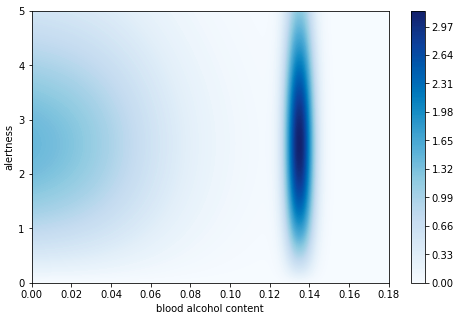
\includegraphics[width=\linewidth]{productivity.png}
    \caption{Productivity function}
    \label{fig:productivity}
\end{figure}

Action space: \emph{just work}, \emph{drink coffee} (increases $s^\text{alert}$ and $s^\text{hypert}$), \emph{drink beer} (decreases $s^\text{alert}$, increases $s^\text{hypert}$ and $s^\text{tox}_t$) and \emph{go to bed} (sleep takes a lot of time, but reduces $s^\text{hypert}$ and $s^\text{tox}_t$ and without it alertness starts to fall very fast)

\begin{figure}[H]
    \centering
    \includegraphics[width=\linewidth]{example.png}
    \caption{Random agent's health indicators}
    \label{fig:random}
\end{figure}

Rewards: small positive for productivity, large negative for a heart attack.

\section{Experiments}
\label{sec:experiments}

We train 2 models (a neural network with 0 hidden layers against one with 3 hidden layers of size 16) with 3 industry-standard algorithms: Cross-Entropy Method, State-Action-Reward-State-Action and Deep Q-Network and compare the resulting agents with a reference strategy of sleep every night followed by a cup of coffee.

We train all models with \texttt{keras-rl}, limiting all episodes to 1000 steps, and test 20 times.
Scores in table \ref{tab:results} are obtained by averaging over total rewards for the 20 test episodes.

\begin{table}[H]
    \centering
    \begin{tabular}{c|c|c|c|c}
         Algorithm & Model & Score & Sleep & Drinks \\
         CEM & 0 & -524.12 &  &   \\
         CEM & 3x16 & -523.88 & & \\
         SARSA & 0 & -130.9 & Yes & \\
         SARSA & 3x16 & -134.95 & Yes & \\
         DQN & 0 & -119.95 & Yes &  \\
         DQN & 3x16 & \textbf{-84.96} & Yes &  \\
         Reference & - & -119.76 & Yes & Yes 
    \end{tabular}
    \caption{Reinforcement learning compared to reference strategy. All models trained to avoid caffeine and alcohol}
    \label{tab:results}
\end{table}

All agents converge to a healthy sleep pattern with no coffee or beer.